\Aufgabe[Predicate Abstraction\hfill\textbf{(1.5 Point)}]
Consider the following program:
\begin{verbatim}
void foo(int j, int z) {
  assume(z != 0);
  int i := j;
  while(z != 0) {
      i := i + z;
      if(z > 0)
          z--
      else
          z ++;
  };
  assert(i != j)
}
\end{verbatim}

The {\em assume statement} at the beginning of the function forces the parameter $z$ not to be 0 when the function is called.

\begin{enumerate}

 \item Argue in your own words why the assertion at the end of the program allways holds, i.e., why the error state can never be reached.

Because of the precondition $assume(z\neq0)$, the while-loop is executed at least one time, no matter of the sign of $z$.
Because of the $if$ - statement inside the loop, the loop is executed exactely $|z|$ - times, with every execution of the loop incrementing or decrementing the variable $i$,
while $j$ is not changed in the program. But because $i=j$ before the loop and the guaranteed execution of loop, $i=j$ cannot hold after the loop.
 \item Provide a labeled transition system for the given program.

\begin{center}
	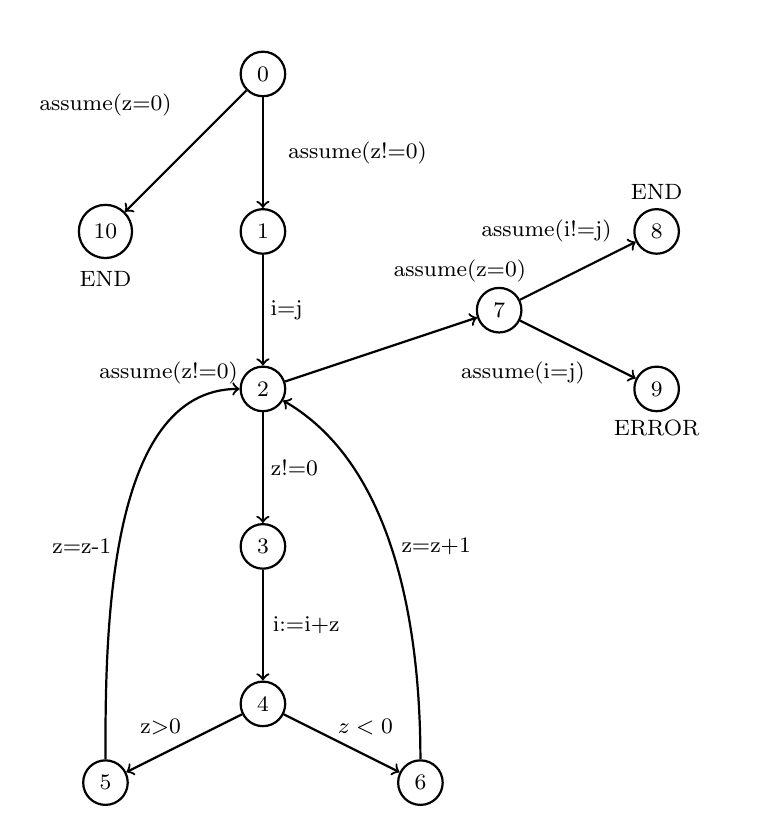
\begin{tikzpicture}[->,scale=1,label distance=0mm,auto]
		\tikzstyle{every node}=[draw,shape=circle,minimum size=5mm,font=\footnotesize];
    \tikzstyle{every path}=[draw,thick];
    \node at (0, 1)   (s0) {$0$};
    \node at (0, -1)  (s1) {$1$};
    \node at (0, -3)  (s2) {$2$};
    \node at (0, -5) (s3) {$3$};
    \node at (0, -7)  (s4) {$4$};
    \node at (-2, -8)  (s5) {$5$};
    \node at (2, -8)  (s6) {$6$};
    \node at (3, -2)  (s7) {$7$};
    \node at (5, -1)  (s8) {$8$};
    \node at (5, -3)  (s9) {$9$};
    \node at (-2, -1)  (s10) {$10$};


\node[draw=none] at (1.2,0) {assume(z!=0)};
\node[draw=none] at (-2,0.6) {assume(z=0)};
\node[draw=none] at (0.3,-2) {i=j};
\node[draw=none] at (0.4,-4) {z!=0};
\node[draw=none] at (0.55,-6) {i:=i+z};
\node[draw=none] at (-1.3,-7.3) {z$>$0};
\node[draw=none] at (1.3,-7.3) {$z<0$};
\node[draw=none] at (-2.3,-5) {z=z-1};
\node[draw=none] at (2.2,-5) {z=z+1};
\node[draw=none,label=right:{}] at (-1.2,-2.8) {assume(z!=0)};
\node[draw=none,label=right:{}] at (2.5,-1.5) {assume(z=0)};

\node[draw=none,label=right:{}] at (-2,-1.6) {END};
\node[draw=none,label=right:{}] at (5,-0.5) {END};
\node[draw=none,label=right:{}] at (5,-3.5) {ERROR};
\node[draw=none,label=right:{}] at (3.6,-1) {assume(i!=j)};
\node[draw=none,label=right:{}] at (3.3,-2.8) {assume(i=j)};


    \draw (s0) to (s10);
    \draw (s0) to (s1);
    \draw (s1) to (s2);
    \draw (s2) to (s3);
    \draw (s2) to (s7);
    \draw (s3) to (s4) ;
    \draw (s4) to (s6) ;
    \draw (s6) .. controls +(up:18mm) and +(330:20mm) .. (s2);
    \draw (s7) to (s8);
    \draw (s7) to (s9);

    \draw (s5) .. controls +(up:18mm) and +(180:20mm) .. (s2);
    \draw (s4) to (s5);
	\end{tikzpicture}
\end{center}



 \item Provide an abstraction for the labeled transition system that uses the predicates $i = j$, $i < j$, $i > j$.

\begin{center}
	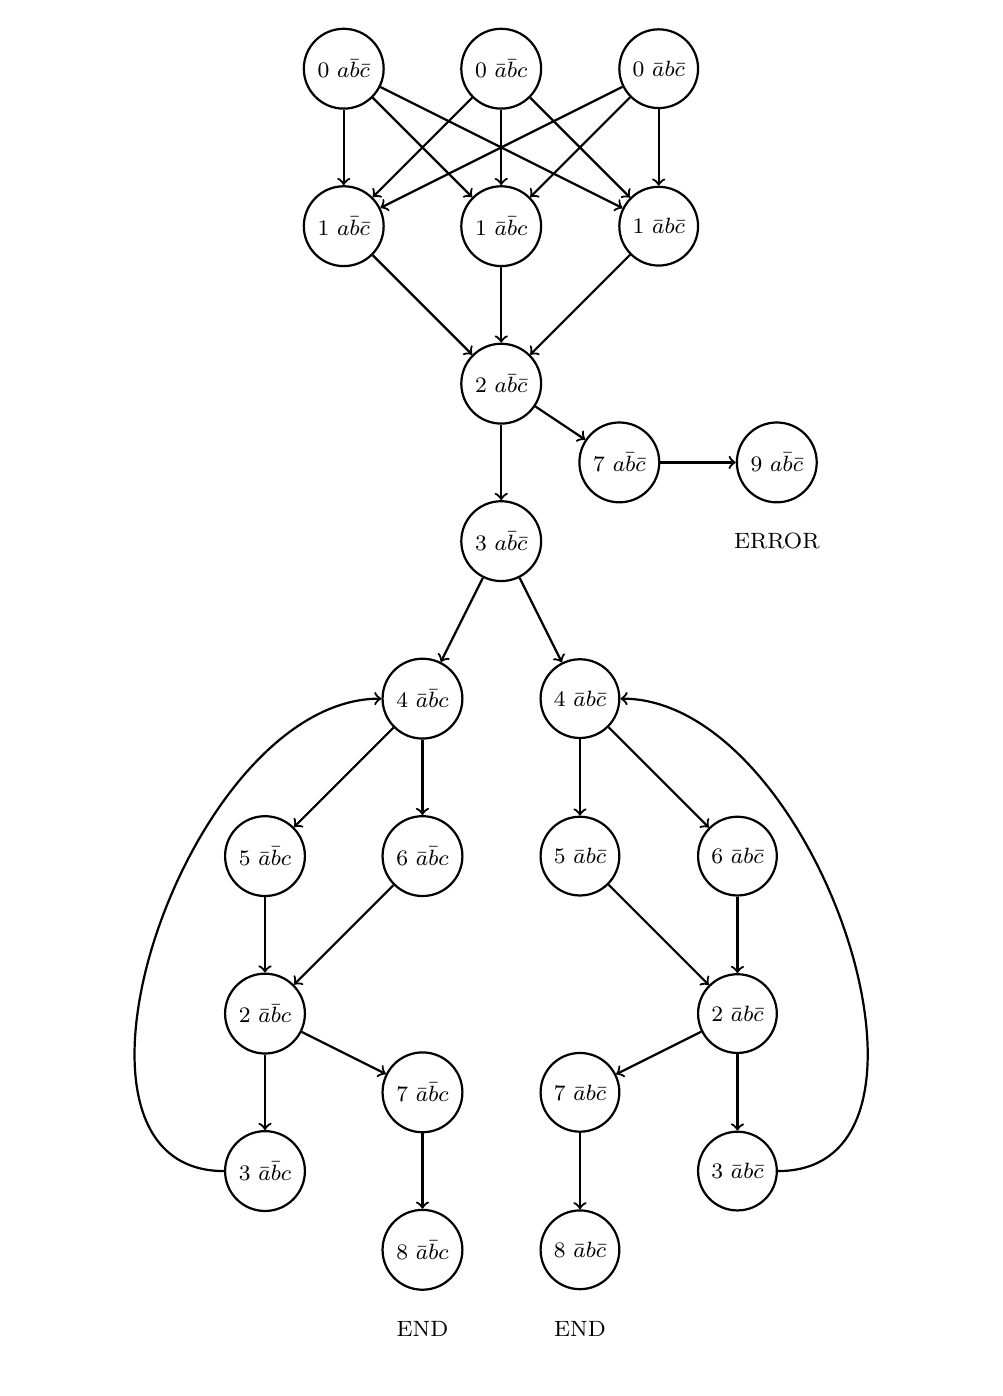
\begin{tikzpicture}[->,scale=1,label distance=0mm,auto]
		\tikzstyle{every node}=[draw,shape=circle,minimum size=10mm,font=\footnotesize];
    \tikzstyle{every path}=[draw,thick];
    \node at (-2, 1)   (sa0) {$0\ a \bar b\bar c$};
    \node at (0, 1)  (sb0) {$0\ \bar a \bar b c$};
    \node at (2, 1)  (sc0) {$0\ \bar a b \bar c$};
	\node at (-2, -1)   (sa1) {$1\ a \bar b\bar c$};
    \node at (0, -1)  (sb1) {$1\ \bar a \bar b c$};
    \node at (2, -1)  (sc1) {$1\ \bar a b\bar c$};
    \node at (0, -3)  (s2) {$2\ a \bar b\bar c$};
    \node at (0, -5)  (s3) {$3\ a \bar b\bar c$};
    \node at (-1, -7)  (s4a) {$4\ \bar a \bar b c$};
    \node at (1, -7)  (s4b) {$4\ \bar a b \bar c$};
	\node at (-3, -9)  (s5a) {$5\ \bar a \bar b c$};
    \node at (-1, -9)  (s6a) {$6\ \bar a \bar b c$};
    \node at (1, -9)  (s5b) {$5\ \bar a b \bar c$};
    \node at (3, -9)  (s6b) {$6\ \bar a b \bar c$};
\node at (-3, -11)  (s2a) {$2\ \bar a \bar b c$};
    \node at (3, -11)  (s2b) {$2\ \bar a b \bar c$};
\node at (-3, -13)  (s3a) {$3\ \bar a \bar b c$};
    \node at (3, -13)  (s3b) {$3\ \bar a b \bar c$};
    \node at (-1, -12)  (s7a) {$7\ \bar a \bar b c$};
    \node at (1, -12)  (s7b) {$7\ \bar a b \bar c$};
  \node at (-1, -14)  (s8a) {$8\ \bar a \bar b c$};
    \node at (1, -14)  (s8b) {$8\ \bar a b \bar c$};
 \node at (1.5, -4)  (s7c) {$7\ a \bar b\bar c$};
    \node at (3.5, -4)  (s9) {$9\ a \bar b\bar c$};
\node[draw=none,label=right:{}] at (3.5,-5) {ERROR};
\draw (s2) to (s7c);
\draw (s7c) to (s9);
\draw (sa0) to (sa1);
\draw (sa0) to (sb1);
\draw (sa0) to (sc1);
\draw (sb0) to (sa1);
\draw (sb0) to (sb1);
\draw (sb0) to (sc1);
\draw (sc0) to (sa1);
\draw (sc0) to (sb1);
\draw (sc0) to (sc1);
\draw (sa1) to (s2);
\draw (sb1) to (s2);
\draw (sc1) to (s2);
\draw (s2) to (s3);
\draw (s3) to (s4a);
\draw (s3) to (s4b);
\draw (s4a) to (s5a);
\draw (s4a) to (s6a);
\draw (s4b) to (s5b);
\draw (s4b) to (s6b);
\draw (s5a) to (s2a);
\draw (s6a) to (s2a);
\draw (s5b) to (s2b);
\draw (s6b) to (s2b);
\draw (s2a) to (s3a);
\draw (s2b) to (s3b);
\draw (s2a) to (s7a);
\draw (s2b) to (s7b);
\draw (s7a) to (s8a);
\draw (s7b) to (s8b);

\draw (s3a) .. controls +(left:30mm) and +(left:30mm) .. (s4a);
\draw (s3b) .. controls +(right:30mm) and +(right:30mm) .. (s4b);

\node[draw=none,label=right:{}] at (-1,-15) {END};
\node[draw=none,label=right:{}] at (1,-15) {END};


	\end{tikzpicture}
\end{center}

 \item Check whether the error state can be reached in the abstraction, if so state a trace to the error state and refine the abstraction with suitable predicates such that the error state is not reachable anymore.

 The error state can  be reached in the abstraction since we don´t have information about z. If we update the abstraction with a predicate for (z != 0) we can be sure that we can´t reach the error state again. 

\begin{center}
	\begin{tikzpicture}[->,scale=1,label distance=0mm,auto]
		\tikzstyle{every node}=[draw,shape=circle,minimum size=10mm,font=\footnotesize];
    \tikzstyle{every path}=[draw,thick];
    \node at (-2, 1)   (sa0) {$0\ a \bar b\bar c$};

    \node at (2, -1)  (sc1) {$1\ \bar a b\bar c$};
    \node at (0, -3)  (s2) {$2\ a \bar b\bar c$};   
    \node at (1.5, -4)  (s7c) {$7\ a \bar b\bar c$};
    \node at (3.5, -4)  (s9) {$9\ a \bar b\bar c$};
\node[draw=none,label=right:{}] at (3.5,-5) {ERROR};

\draw (s2) to (s7c);
\draw (s7c) to (s9);
\draw (sa0) to (sc1);
\draw (sc1) to (s2);
\draw (s2) to (s3);

\end{tikzpicture}
\end{center}



\end{enumerate}
